\capitulo{3}{Conceptos teóricos}

En este capitulo se han recogido algunos conocimientos básicos sobre los \emph{Mixing Models} que son necesarios para enmarcar el problema. Además tenemos como objetivo explicar el problema que se resuelve con la aplicación.

\section{Mixing Models}

Los modelos de mezcla (\emph{Mixing Models}) son herramientas estadísticas que utilizan biotrazadores para estimar las contribuciones de diversas fuentes a una mezcla.
Estas herramientas son usadas en muchos problemas. A continuación se expondrán algunos ejemplos donde se usan los \emph{Mixing Models}:

%\clearpage

\textbf{La dieta en la ecología}

La dieta en ecología  (fuentes = presas, mezcla = dieta de un consumidor). En el ejemplo de la Figura \ref{fig:preyDiet} se usan los \emph{Mixing Models} para calcular las contribuciones de diferentes presas del entorno (p. ej. mamíferos marinos, salmones, ciervos) a la dieta de un depredador (p. ej. Lobo) a partir de la composición de sus heces. En el articulo \cite{improveBayes2009} se resuelve este problema usando MixSir y se obtuvieron resultados robustos. Por último, Jackson et al. (2009) propone añadir parámetros de error adicionales al ámbito de la mezcla .

\begin{figure}[h!] 
\centering
    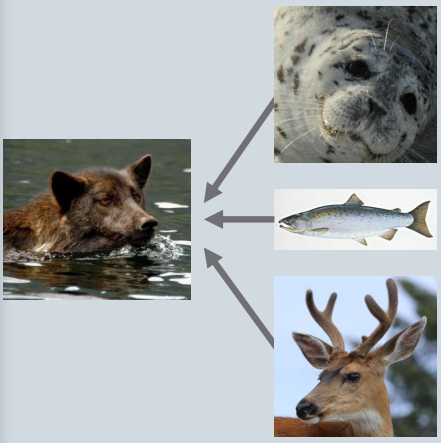
\includegraphics[width=0.8\textwidth]{img/preyDiet.PNG}
\caption{Ejemplo dieta en ecología }
\label{fig:preyDiet}
\end{figure}

\clearpage

\textbf{Movimiento en ecología}

Los modelos de mezcla también se utilizan en ecología para estimar movimientos de animales (fuentes = regiones, mezcla =  animales que pueden desplazarse entre regiones). Estos modelos son usados por ecologistas para calcular composiciones de comunidades y la biodiversidad a nivel de sitio terrestre de todo el mundo.

artículo: \url{https://onlinelibrary.wiley.com/doi/full/10.1002/ece3.1303}

\begin{figure}[h!] 
\centering
    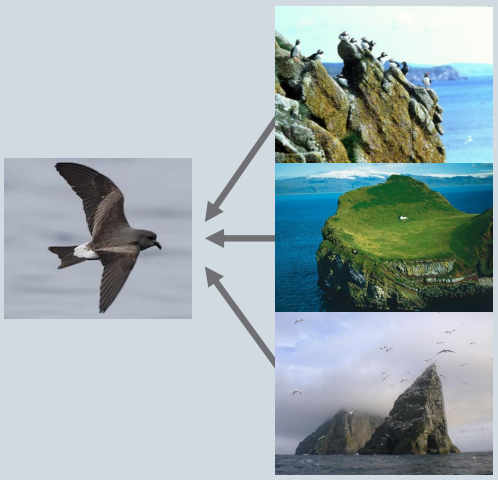
\includegraphics[width=0.8\textwidth]{img/colonyBird.PNG}
\caption{Ejemplo Movimiento en ecología }
\label{fig:colonyBird}
\end{figure}

\clearpage

\textbf{Sedimentos en sistemas fluviales}

Sedimentos en sistemas fluviales (fuentes = terrenos aguas arriba, mezcla = sedimentos aguas abajo). El objetivo de los sistemas de agricultura regenerativa (Rodale, 1983) es aumentar la calidad del suelo y la biodiversidad de las tierras de labranza, favoreciendo la creación de productos agrícolas nutritivos de forma rentable.

%TODO: \url{https://peerj.com/articles/4428/}
artículo: \url{https://pubmed.ncbi.nlm.nih.gov/30812003/}

\begin{figure}[h!] 
\centering
    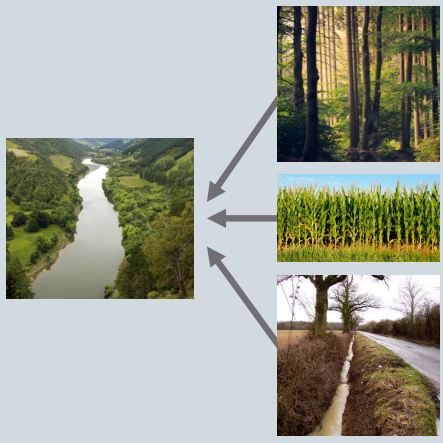
\includegraphics[width=0.8\textwidth]{img/soilSediment.PNG}
\caption{Ejemplo Sedimentos en sistemas fluviales }
\label{fig:soilSediment}
\end{figure}


\clearpage

\subsection{Cómo funcionan los \emph{Mixing Models}}

Comenzamos explicando un problema sencillo. El problema se plantea dadas dos fuentes posibles de alimentos (Source 1, Source 2) y un consumidor (ver fig. \ref{fig:workMixing0}). Nuestro objetivo es identificar la dieta del consumidor a partir de la composición de sus heces. Para ello, se hace uso de biotrazadores o marcadores, que se encuentran presentes en las fuentes y no se alteran en el proceso de digestión. De esta forma, los biotrazadores nos permiten realizar estimaciones de la cantidad de cada una de las fuentes que puede haber ingerido un consumidor. 

\begin{figure}[h!] 
\centering
    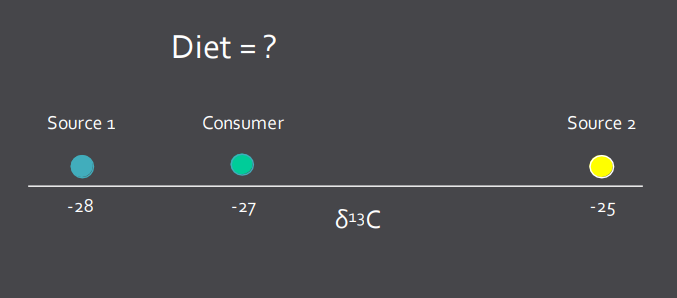
\includegraphics[width=0.8\textwidth]{img/workMixing0.PNG}
\caption{Linear \emph{Mixing Models} - Problema }
\label{fig:workMixing0}
\end{figure}

Para simplificar la explicación supondremos que la masa se conserva durante el proceso de digestión, por ello partimos de la ecuación $p_1 + p_2 = 1$, donde $p_i$ denota la masa de fuente (\emph{source}) $i$ por cada unidad de masa de heces. Como suponemos que la masa se conerva, la suma de las proporciones de las fuentes es igual a 1. Tenemos también una segunda ecuación que refleja la conservación de la masa del biotrazador \textdelta$_{13}C$ a través del proceso de digestión: $Consumer = p_1*S_1 + p_2*S_2$, donde $Consumer$ es la masa de biotrazador en las heces, y $S_i$ denota la concentración de biotrazador en la fuente $i$.

\begin{figure}[h!] 
\centering
    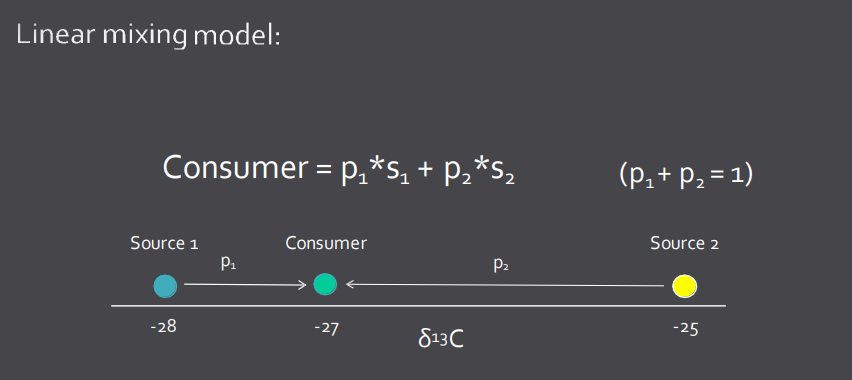
\includegraphics[width=0.8\textwidth]{img/workMixing1.PNG}
\caption{Linear \emph{Mixing Models} - Ecuaciones con un marcador }
\label{fig:workMixing1}
\end{figure}

En el caso de la figura \ref{fig:workMixing1} solo teníamos un eje / biotrazador / marcador, por lo que solo considerábamos una ecuación. En el figura \ref{fig:workMixing2} tenemos dos ejes para los biotrazadores: \textdelta$_{13}C$ y \textdelta$_{15}N$, además de una fuente más ($S_1$, $S_2$, $S_3$). En consecuencia, podemos usar las siguientes ecuaciones: 

$$ Consumer_C = p_1*S_{1C} + p_2*S_{2C} + p_3*S_{3C} $$
$$ Consumer_N = p_1*S_{1N} + p_2*S_{2N} + p_3*S_{3N} $$
$$ p_1 + p_2 = 1 $$

Siendo $S_{iN}$ la concentración del segundo biotrazador  (\textdelta$_{15}N$) en la fuente $i$,  y ese valor se multiplicara por la proporción de la fuente $i$ que se ha ingerido.

\begin{figure}[h!] 
\centering
    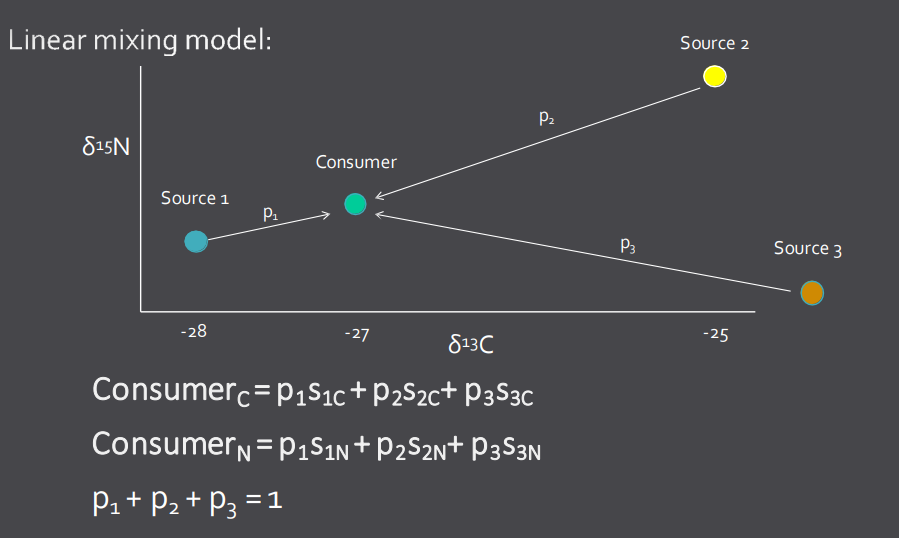
\includegraphics[width=0.8\textwidth]{img/workMixing2.PNG}
\caption{Linear \emph{Mixing Models} - Ecuaciones con dos marcadores }
\label{fig:workMixing2}
\end{figure}

%\subsection{}

En el caso de mi aplicación, se diseñó sin imponer la condición de conservación de la masa. Esto ha ofrecido un mayor realismo a los cálculos de la aplicación, ya que en general la masa de las heces no coincide necesariamente con la suma de las masas que se ingieren (p. ej. los alimentos ingeridos suelen tener más concentración de agua que las heces).

\newpage

	



